\documentclass[11pt, a4paper]{article}

% ── Encoding & fonts ──────────────────────────────────────────
\usepackage[T1]{fontenc}
\usepackage[utf8]{inputenc}
\usepackage{lmodern}   % vector CM fonts — fixes ligature rendering in PDF

% ── Page layout ───────────────────────────────────────────────
\usepackage[top=2.5cm, bottom=2.5cm, left=2.5cm, right=2.5cm]{geometry}
\usepackage{setspace}
\onehalfspacing

% ── Math ──────────────────────────────────────────────────────
\usepackage{amsmath, amssymb, amsthm}
\usepackage{mathtools}
\usepackage{bm}

% ── Tables & Figures ──────────────────────────────────────────
\usepackage{booktabs}
\usepackage{multirow}
\usepackage{graphicx}
\usepackage{float}
\usepackage{caption}
\usepackage{subcaption}

% ── Colors & Hyperlinks ──────────────────────────────────────
\usepackage[dvipsnames]{xcolor}
\usepackage{hyperref}
\hypersetup{
    colorlinks = true,
    linkcolor  = NavyBlue,
    citecolor  = NavyBlue,
    urlcolor   = NavyBlue,
}

% ── Code listings (for deployment section) ────────────────────
\usepackage{listings}
\lstset{
  basicstyle=\ttfamily\small,
  backgroundcolor=\color{gray!8},
  frame=single,
  framerule=0pt,
  breaklines=true,
  columns=fullflexible,
}

% ── Headers ───────────────────────────────────────────────────
\usepackage{fancyhdr}
\pagestyle{fancy}
\fancyhf{}
\rhead{\textcolor{gray}{\small \rightmark}}
\lhead{\textcolor{gray}{\small Credit Risk Scoring Pipeline}}
\cfoot{\thepage}
\renewcommand{\headrulewidth}{0.4pt}

% ── Figure path ───────────────────────────────────────────────
\graphicspath{{figures/}}

% ── BibLaTeX Configuration ────────────────────────────────────
\usepackage[
  backend=biber,
  style=authoryear,
  sorting=nyt,
  citestyle=authoryear,
  bibstyle=authoryear,
  maxcitenames=2,
  maxbibnames=99
]{biblatex}
\addbibresource{references.bib}

% ── Custom commands ───────────────────────────────────────────
\newcommand{\PD}{\text{PD}}
\newcommand{\LGD}{\text{LGD}}
\newcommand{\EAD}{\text{EAD}}
\newcommand{\EL}{\text{EL}}

% ── Document Metadata ─────────────────────────────────────────
\title{%
  \vspace{-1cm}
  {\Large\bfseries Credit Risk Scoring Pipeline}\\[0.3cm]
  {\large Machine Learning Models, Regulatory Compliance,\\
  and Deployed Scoring Application}\\[0.5cm]
  {\normalsize Technical Report}
}
\author{%
  Credit Risk Pipeline Project\\
  {\small Applied and Computational Mathematics}\\
  {\small\texttt{github.com/credit-risk-pipeline}}
}
\date{April 2026}

\begin{document}

\maketitle
\thispagestyle{fancy}

% ============================================================================
% ABSTRACT
% ============================================================================
\begin{abstract}
\noindent
This report presents an end-to-end machine learning pipeline for credit risk scoring, built on the Home Credit Default Risk dataset of 307,511 loan applications across seven relational tables. A total of 169 features are engineered from the multi-table data using credit-domain aggregations (affordability ratios, delinquency counts and means across bureau and installment records, composite external scores). Three gradient boosting models (XGBoost, LightGBM, and CatBoost) are trained using out-of-time validation that follows the Basel Committee on Banking Supervision temporal validation requirements. The production CatBoost model achieves an out-of-time Gini coefficient of 0.5814 (AUC-ROC 0.7907, KS statistic 0.4147), against a logistic regression baseline Gini of 0.4681 on the same split (a 24.2\% improvement). Fairness analysis finds no statistically significant gender-based disparate impact (Disparate Impact Ratio 0.955, above the 0.80 threshold). SHAP-based local explanations are produced for each prediction to support adverse action notices under GDPR Article 22. Regulatory compliance is assessed against the Basel III IRB framework, GDPR Article 22 on automated decision-making, the EU Artificial Intelligence Act (Regulation 2024/1689), and the EU Consumer Credit Directive (Directive 2023/2225). The production system is deployed as a FastAPI scoring endpoint and a Streamlit interactive dashboard.

\medskip
\noindent
\textbf{Keywords:} credit scoring, probability of default, gradient boosting, SHAP, Basel III IRB, EU AI Act, class imbalance, model calibration
\end{abstract}

\tableofcontents
\newpage

% ============================================================================
% 1. INTRODUCTION
% ============================================================================
\section{Introduction}
\label{sec:introduction}

Credit risk assessment is central to banking operations. The probability that a borrower fails to meet contractual obligations drives capital allocation, loan pricing, and portfolio provisioning. Altman's \citeyear{altman1968} discriminant analysis model introduced the Z-score for bankruptcy prediction, and Merton's \citeyear{merton1974} structural model formalized default as the event that a firm's asset value falls below its debt obligations at maturity. Statistical scoring and structural default modeling are the two conceptual bases of modern credit risk practice.

In contemporary retail lending, probability of default (PD) estimation is typically performed using statistical or machine learning classifiers trained on historical loan performance data. The PD estimate feeds directly into the Expected Loss formula,
\begin{equation}
\label{eq:expected_loss}
\EL = \PD \times \LGD \times \EAD,
\end{equation}
where Loss Given Default ($\LGD$) and Exposure at Default ($\EAD$) are estimated separately. Under the Basel III Internal Ratings-Based (IRB) approach \parencite{bcbs_basel_framework_2024}, banks that develop internal PD models may use them for regulatory capital calculations, subject to strict validation requirements.

Recent EU legislation imposes new obligations on credit scoring models. The EU Artificial Intelligence Act (Regulation 2024/1689) classifies AI systems used for credit scoring as high-risk \parencite{eu_ai_act_2024_1689}, requiring transparency, human oversight, and bias testing. The EU Consumer Credit Directive (Directive 2023/2225) mandates that when creditworthiness assessment involves automated processing, consumers have the right to human intervention and a meaningful explanation of the assessment \parencite{eu_consumer_credit_directive_2023}. Model explainability and fairness auditing are therefore regulatory requirements.

This work develops a calibrated PD model on the Home Credit Default Risk dataset, a multi-table relational dataset with approximately 8\% default rate. Three gradient boosting architectures (XGBoost, LightGBM, CatBoost) are compared against a logistic regression baseline. The best single model (CatBoost, out-of-time Gini = 0.5814) is paired with SHAP-based explainability \parencite{lundberg2017} to meet regulatory requirements. The contribution is twofold: (1) a methodologically sound pipeline with temporal validation compliant with Basel requirements, and (2) a deployed production system combining calibrated PD estimation with per-applicant SHAP attribution and fairness auditing across protected attributes.

% ============================================================================
% 2. THEORETICAL BACKGROUND
% ============================================================================
\section{Theoretical Background}
\label{sec:theory}

\subsection{From Altman's Z-Score to Machine Learning Scorecards}

The statistical approach to credit risk prediction originates with Altman's \citeyear{altman1968} multiple discriminant analysis model. Using a sample of 66 manufacturing firms (33 bankrupt, 33 non-bankrupt), Altman derived a linear discriminant function of the form
\begin{equation}
\label{eq:altman_z}
Z = v_1 X_1 + v_2 X_2 + \cdots + v_n X_n,
\end{equation}
where $X_1, \ldots, X_n$ are financial ratios (working capital to total assets, retained earnings to total assets, EBIT to total assets, market equity to book debt, and sales to total assets) and $v_1, \ldots, v_n$ are discriminant coefficients. The model achieved 93.5\% classification accuracy on the original sample and established that multivariate ratio analysis could predict corporate failure up to two years before the event \parencite{altman1968}.

In modern retail credit scoring, the same principle applies at the individual borrower level: a set of applicant characteristics (income, employment history, prior delinquencies, credit bureau scores) is mapped to a default probability. The transition from Altman's corporate discriminant function to consumer credit models has been accompanied by a shift in methodology, from linear discriminant analysis and logistic regression toward tree-based ensemble methods such as XGBoost \parencite{chen2016xgboost} and LightGBM, which capture non-linear relationships and feature interactions without manual specification.

\subsection{The Merton Structural Model and Probability of Default}

Merton's \citeyear{merton1974} structural model provides the theoretical basis for understanding default as a financial event. The model treats a firm's equity as a European call option on its asset value $A$, with the face value of debt $F$ as the strike price and the debt maturity $T$ as the expiration date. Default occurs when the firm's asset value at maturity falls below its debt obligations:
\begin{equation}
\label{eq:merton_default}
\Pr[\text{Default}] = \Pr[A_T < F] = \Phi\!\left(\frac{\ln(F/A_0) - (\mu - \tfrac{1}{2}\sigma^2)T}{\sigma\sqrt{T}}\right),
\end{equation}
where $\Phi$ is the standard normal CDF, $\mu$ is the expected return on assets, and $\sigma$ is the asset volatility \parencite{merton1974}. In the Basel II/III IRB framework, this structural insight is formalized through the Vasicek single-factor model, which determines the regulatory risk weight function:
\begin{equation}
\label{eq:irb_rwa}
K(\PD) = \Phi\!\left(\frac{\Phi^{-1}(\PD) + \sqrt{\rho(\PD)}\,\Phi^{-1}(0.999)}{\sqrt{1 - \rho(\PD)}}\right) - \PD,
\end{equation}
where $\rho(\PD)$ is an asset correlation parameter interpolated between 12\% and 24\% as a function of PD \parencite{bluhm2010, bcbs_basel_framework_2024}. The risk-weighted assets are then
\begin{equation}
\text{RWA} = 12.5 \times \EAD \times \LGD \times K(\PD) \times M(\PD, \text{MAT}),
\end{equation}
where $M$ is a maturity adjustment. PD estimation is therefore more than a classification exercise. The PD value enters directly into capital calculations, so calibration errors propagate to regulatory capital.

While Merton's model applies to corporate credit (where equity and asset values are observable or estimable), the consumer credit setting lacks a corresponding asset process. In retail portfolios, PD is estimated empirically from historical default data, typically using logistic regression or tree-based classifiers. The connection to Merton remains conceptual: borrower creditworthiness (the ``distance to default'') is inferred from observable features rather than from an explicit asset value model.

\subsection{Gradient Boosted Trees for Credit Scoring}

Gradient boosted decision trees have become the dominant method for tabular prediction problems, including credit scoring. XGBoost, introduced by Chen and Guestrin \citeyear{chen2016xgboost}, formulates tree boosting as the minimization of a regularized objective:
\begin{equation}
\label{eq:xgboost_obj}
\mathcal{L}(\phi) = \sum_{i=1}^{n} \ell(y_i, \hat{y}_i) + \sum_{k=1}^{K} \Omega(f_k),
\end{equation}
where $\ell$ is a differentiable loss function (typically log-loss for binary classification), $f_k$ are individual trees, and $\Omega(f_k) = \gamma T_k + \tfrac{1}{2}\lambda \lVert w_k \rVert^2$ penalizes model complexity through the number of leaves $T_k$ and the leaf weight magnitude $\lVert w_k \rVert^2$ \parencite{chen2016xgboost}. The algorithm builds trees greedily, using a second-order Taylor expansion of the loss at each split, which enables efficient computation of optimal split points.

For credit scoring, gradient boosted trees have several practical advantages over logistic regression. They handle missing values natively, which matters substantially when 45\% to 55\% of external credit scores are missing. They also capture non-linear effects and interactions between features without manual engineering, and they tolerate moderate multicollinearity in the feature set. The trade-off is reduced interpretability, which is why post-hoc explainability methods such as SHAP values are needed.

\subsection{SHAP: Model-Agnostic Explainability}

SHAP (SHapley Additive exPlanations), introduced by Lundberg and Lee \citeyear{lundberg2017}, provides a unified framework for interpreting predictions by assigning each feature an importance value based on cooperative game theory. For a prediction $f(x)$ on input $x$, the SHAP value for feature $j$ is
\begin{equation}
\label{eq:shap}
\phi_j(f, x) = \sum_{S \subseteq N \setminus \{j\}} \frac{|S|!\,(|N| - |S| - 1)!}{|N|!} \bigl[f(x_{S \cup \{j\}}) - f(x_S)\bigr],
\end{equation}
where $N$ is the set of all features and $f(x_S)$ denotes the expected model output when only features in $S$ are known \parencite{lundberg2017}. SHAP values satisfy three properties: local accuracy (the sum of SHAP values plus the base value equals the prediction), missingness (absent features receive zero attribution), and consistency (if a feature's marginal contribution increases, its SHAP value does not decrease).

For tree-based models, TreeExplainer computes exact SHAP values in polynomial time, with complexity $O(TLD^2)$ where $T$ is the number of trees, $L$ is the maximum number of leaves, and $D$ is the maximum depth. This makes SHAP tractable for production credit models with thousands of trees. In the regulatory context, SHAP values translate directly into adverse action factors: the top features with negative SHAP values (increasing default probability) form the required explanation of an unfavorable credit decision under GDPR Article 22(3).

\subsection{Regulatory Framework}
\label{subsec:regulatory_framework}

The regulatory environment for credit scoring models in the EU rests on three pillars.

\paragraph{Basel III IRB Approach.} Under the Capital Requirements Regulation (CRR, Articles 142 to 191), institutions using internal PD models for capital calculations must satisfy extensive validation requirements \parencite{crr_irb_2013}. Article 144(1) requires that rating systems provide ``a meaningful assessment of obligor and transaction characteristics, a meaningful differentiation of risk and accurate and consistent quantitative estimates of risk.'' The ECB Guide to Internal Models further specifies that institutions must demonstrate at least three years of use in risk management and credit approval processes before receiving IRB approval \parencite{ssm_guide_2025}. Temporal (out-of-time) validation is a requirement for ensuring that model performance estimates are not contaminated by look-ahead bias.

\paragraph{EU Artificial Intelligence Act (Regulation 2024/1689).} The AI Act classifies credit scoring as a high-risk AI system under Annex III, Point 5(b) \parencite{eu_ai_act_2024_1689}. Providers of such systems must satisfy requirements on data governance (Article 10), transparency (Article 13), human oversight (Article 14), and accuracy, robustness, and cybersecurity (Article 15). Market surveillance is coordinated between national competent authorities and, for significant credit institutions within the Single Supervisory Mechanism, the ECB.

\paragraph{EU Consumer Credit Directive (Directive 2023/2225).} The Directive states that ``whenever the creditworthiness assessment involves automated processing, the consumer should have the right to obtain human intervention on the part of the creditor'' and ``a meaningful, comprehensible explanation of the assessment made and of the functioning of the automated processing used, including the main variables, the logic and risks involved'' \parencite{eu_consumer_credit_directive_2023}. This requirement makes feature attribution methods such as SHAP values a practical necessity for compliance.

% ============================================================================
% 3. DATA DESCRIPTION
% ============================================================================
\section{Data Description}
\label{sec:data}

The Home Credit Default Risk dataset contains 307,511 loan applications from an online lending company, organized into seven relational tables. The core \texttt{application\_train/test} table stores applicant demographics (age, employment tenure, family status), loan characteristics (credit amount, annuity, goods price), and document submission flags. Six secondary tables capture the applicant's credit history: \texttt{bureau} (credit bureau records from external agencies), \texttt{bureau\_balance} (monthly payment history for bureau accounts), \texttt{previous\_application} (prior loan records at Home Credit), \texttt{POS\_CASH\_balance} (point-of-sale cash balance history), \texttt{installments\_payments} (installment payment records), and \texttt{credit\_card\_balance} (credit card statement history).

The target variable is a binary indicator: default (TARGET = 1) within 30 days of loan origination. Approximately 8\% of applications default, producing a class imbalance ratio of roughly 1:11.5. Three external credit bureau scores (EXT\_SOURCE\_1, EXT\_SOURCE\_2, EXT\_SOURCE\_3) are the strongest individual predictors but exhibit 45\% to 55\% missingness. This missing data pattern is structural: not all applicants have records in all external bureaus. The missingness itself carries predictive signal (applicants without external scores may be thinner-file borrowers), which motivates the use of sentinel imputation rather than deletion or mean imputation.

The multi-table structure of this dataset is deliberate. In production credit scoring, applicant data arrives from application forms, internal records, and external bureaus, so joining and aggregating features across relational sources is part of the job. Single-table datasets do not test this capability.

% ============================================================================
% 4. METHODOLOGY
% ============================================================================
\section{Methodology}
\label{sec:methodology}

\subsection{Feature Engineering}

Raw features from the seven tables were engineered into 169 base features across 12 categories: applicant demographics (age in years, employment tenure), loan affordability ratios (credit-to-income, annuity-to-income), delinquency aggregates from secondary tables (count, mean, max, and standard deviation of days past due across bureau and installment records), and composite external scores (EXT\_SOURCE\_MEAN and EXT\_SOURCE\_MIN computed using robust aggregation to handle missing values).

Division-by-zero protection was applied to all ratio features: values were clipped to $[0, \infty)$, infinities replaced by zero, and NaN values filled with a tree-friendly sentinel of $-999$. Sentinel imputation is preferred over population-mean imputation for tree-based models because the tree can learn a dedicated split for sentinel values, which treats ``missing'' as a separate category. In credit data the missingness pattern itself carries predictive signal, and sentinel imputation preserves that signal.

No Weight of Evidence (WoE) discretization was applied. WoE encoding is standard for logistic regression scorecards and is favored for interpretability, but it discards information about within-bin variation. Raw continuous features allow tree-based models to learn optimal split points directly from the data; in the benchmark reported in Section~\ref{sec:results}, raw features produced a higher OOT Gini than WoE-encoded inputs (CatBoost at 0.5814 against XGBoost-WoE at 0.5519).

\subsection{Validation Strategy: Out-of-Time Testing}

All models were trained using a validation protocol designed to satisfy Basel temporal validation requirements:

\begin{enumerate}
  \item \textbf{Sort by application ID.} The full dataset was sorted by SK\_ID\_CURR (loan ID) in chronological order, with random permutation of NaN rows seeded by cross-fold index for reproducibility.
  \item \textbf{Carve out-of-time (OOT) set.} The most recent 20\% of records (approximately 61,502 applications) were set aside as a frozen OOT test set. This set was never exposed to hyperparameter optimization or feature selection.
  \item \textbf{Hyperparameter search on training data.} Optuna-based Bayesian hyperparameter optimization was conducted on the remaining 80\% (approximately 246,009 applications), using temporal $k$-fold cross-validation with a 2\% embargo period between folds to prevent serial-correlation leakage.
  \item \textbf{Retrain with selected hyperparameters.} The best hyperparameters (selected by out-of-fold Gini coefficient) were used to retrain the model on the full 80\% training set without further tuning.
  \item \textbf{Evaluate on frozen OOT set.} Final evaluation was performed on the frozen OOT set; these metrics serve as the regulatory evidence of model performance.
\end{enumerate}

The embargo period in step 3 prevents information leakage through serial correlation in temporal features. If fold $k$ ends at time $t$, then fold $k+1$ begins at time $t + \Delta$, where $\Delta$ corresponds to 2\% of the training data. This approach follows the purging and embargo methodology described by de Prado \citeyear{deprado2018} for financial machine learning, adapted to the cross-sectional credit setting.

\subsection{Model Training}

Three gradient boosting architectures were trained: XGBoost \parencite{chen2016xgboost}, LightGBM, and CatBoost. In addition, a logistic regression baseline with WoE-encoded features was trained for comparison. All tree-based models used cost-sensitive weighting to address the 8\% default prevalence:
\begin{equation}
w_i = \begin{cases}
n_{\text{neg}} / n_{\text{pos}} & \text{if } y_i = 1 \text{ (default)}\\
1 & \text{if } y_i = 0 \text{ (non-default)}
\end{cases}
\end{equation}
This weighting upweights the minority class in the loss function, so the model learns the default boundary from the original samples rather than from synthetic ones. Alternative approaches (SMOTE oversampling, threshold adjustment) were evaluated but produced lower KS statistics on the OOT set.

Probability calibration was applied post-hoc to all models using Platt scaling \parencite{niculescu2005predicting}. A separate calibration holdout (30\% of the training data) was carved before hyperparameter optimization and kept entirely separate from both the training folds and the OOT set. Calibration is needed because cost-sensitive weighting distorts the predicted probability distribution: a model trained with balanced class weights produces probabilities centered around 0.5 rather than around the true prevalence of 0.08. Platt scaling fits a logistic regression from raw model outputs to observed outcomes and corrects this shift.

\subsection{Evaluation Metrics}

Four metrics were computed for all models on the frozen OOT set:

\paragraph{Gini coefficient.} Defined as $\text{Gini} = 2 \times \text{AUC} - 1$, the Gini coefficient measures discrimination power and is the standard metric in credit scoring. A Gini of 0 indicates random performance; a Gini of 1 indicates perfect separation of defaults and non-defaults. Industry-grade retail credit scorecards typically achieve Gini values between 0.50 and 0.80; values above 0.70 are considered strong for consumer credit.

\paragraph{KS statistic.} The Kolmogorov-Smirnov statistic measures the maximum vertical distance between the cumulative distribution functions of default and non-default scores:
\begin{equation}
\text{KS} = \max_s \bigl|F_1(s) - F_0(s)\bigr|,
\end{equation}
where $F_1$ and $F_0$ are the CDFs for defaulters and non-defaulters, respectively. The KS statistic captures separation at the tail of the score distribution, which is particularly relevant for pricing and risk stratification decisions.

\paragraph{Brier score.} The mean squared error of predicted probabilities against observed binary outcomes:
\begin{equation}
\text{Brier} = \frac{1}{n}\sum_{i=1}^{n}(\hat{p}_i - y_i)^2.
\end{equation}
Lower Brier scores indicate better calibration. Because PD estimates feed directly into Expected Loss calculations (Equation~\ref{eq:expected_loss}), calibration accuracy has direct regulatory and business consequences.

\paragraph{AUC-ROC.} The area under the receiver operating characteristic curve, measuring the probability that a randomly chosen defaulter receives a higher predicted score than a randomly chosen non-defaulter.

\subsection{Explainability and Fairness}

SHAP TreeExplainer values were computed for the production CatBoost model to decompose each predicted probability by feature contribution. Global SHAP analysis (beeswarm and bar plots) identifies the most influential features across the entire portfolio. Local SHAP analysis (waterfall and force plots) provides per-applicant explanations, supporting adverse action notice generation under GDPR Article 22(3) and the EU Consumer Credit Directive's requirement for a meaningful explanation of automated assessments.

Fairness was audited using the Disparate Impact Ratio (DIR), defined as
\begin{equation}
\text{DIR} = \frac{P(\hat{Y} = 1 \mid \text{group} = \text{protected})}{P(\hat{Y} = 1 \mid \text{group} = \text{privileged})}.
\end{equation}
The 80\% threshold (DIR $\geq$ 0.80), derived from U.S. EEOC employment discrimination guidelines and adopted as a reference standard in the EU context, was applied. Values below 0.80 indicate potential disparate impact. Fairness was evaluated separately for gender (binary: M/F) and age (ternary: Young under 35, Middle 35 to 55, Senior above 55). Age was excluded from the model's training features as a fairness mitigation strategy.

% ============================================================================
% 5. RESULTS
% ============================================================================
\section{Results and Comparison}
\label{sec:results}

\subsection{Model Benchmark}

Five credit risk models were trained and evaluated on the frozen OOT set. The results are reported in Table~\ref{tab:benchmark}.

\begin{table}[H]
  \centering
  \caption{Multi-model benchmark: OOT performance metrics (temporal validation, chronological sort by SK\_ID\_CURR). CatBoost v2 achieves the highest Gini coefficient (0.5814) and AUC-ROC (0.7907). Baseline: Logistic Regression with WoE-encoded features. Tree models use raw continuous features with cost-sensitive weighting and Platt scaling calibration.}
  \label{tab:benchmark}
  \begin{tabular}{lcccc}
    \toprule
    Model & Gini & KS & Brier & AUC-ROC \\
    \midrule
    Logistic Regression (WoE)\textsuperscript{a} & 0.4681 & 0.3486 & 0.1495\textsuperscript{b} & 0.7340 \\
    XGBoost (WoE) & 0.5519 & 0.4159 & 0.0672 & 0.7734 \\
    LightGBM v2 & 0.5695 & 0.4346 & 0.0682 & 0.7848 \\
    CatBoost DFS & 0.5608 & 0.4275 & 0.0659 & 0.7804 \\
    \textbf{CatBoost v2 (Production)} & \textbf{0.5814} & \textbf{0.4147} & \textbf{0.0662} & \textbf{0.7907} \\
    \bottomrule
  \end{tabular}
\end{table}

The production CatBoost model achieves a Gini of 0.5814, representing a 24.2\% improvement over the logistic regression baseline (Gini 0.4681). All tree-based models outperform the logistic regression baseline, confirming the benefit of capturing non-linear feature interactions through gradient boosting ensembles.

\smallskip
\noindent\textsuperscript{a}\,All models are evaluated on the identical out-of-time test set (most-recent 20\% sorted by \texttt{prev\_days\_decision\_mean}), ensuring a like-for-like comparison.
\textsuperscript{b}\,The logistic regression Brier score is high (0.1495) because the model is uncalibrated: it was trained on a dataset with 8\% default prevalence, whereas the OOT window contains 6.2\% defaults. Discrimination metrics (Gini, KS, AUC-ROC) are unaffected by this miscalibration and remain directly comparable.

Two observations are worth noting. First, LightGBM v2 achieves the highest KS statistic (0.4346) among all models, indicating stronger separation at the tail of the score distribution. This property is useful for pricing and risk stratification, where the focus is on distinguishing high-risk from moderate-risk applicants. Second, the OOT and out-of-fold (OOF) Gini gap for the production CatBoost model is only 0.028, indicating stable generalization with modest in-sample optimism.

The logistic regression baseline uses WoE-encoded categorical features and serves two purposes: it establishes a performance floor for comparison, and it represents the type of model that regulators are most familiar with. In a production setting, a ``champion/challenger'' framework would run both the ML model and the logistic regression baseline in parallel, using the latter as a fallback and regulatory reference.

\subsection{Model Performance Visualizations}

\begin{figure}[H]
  \centering
  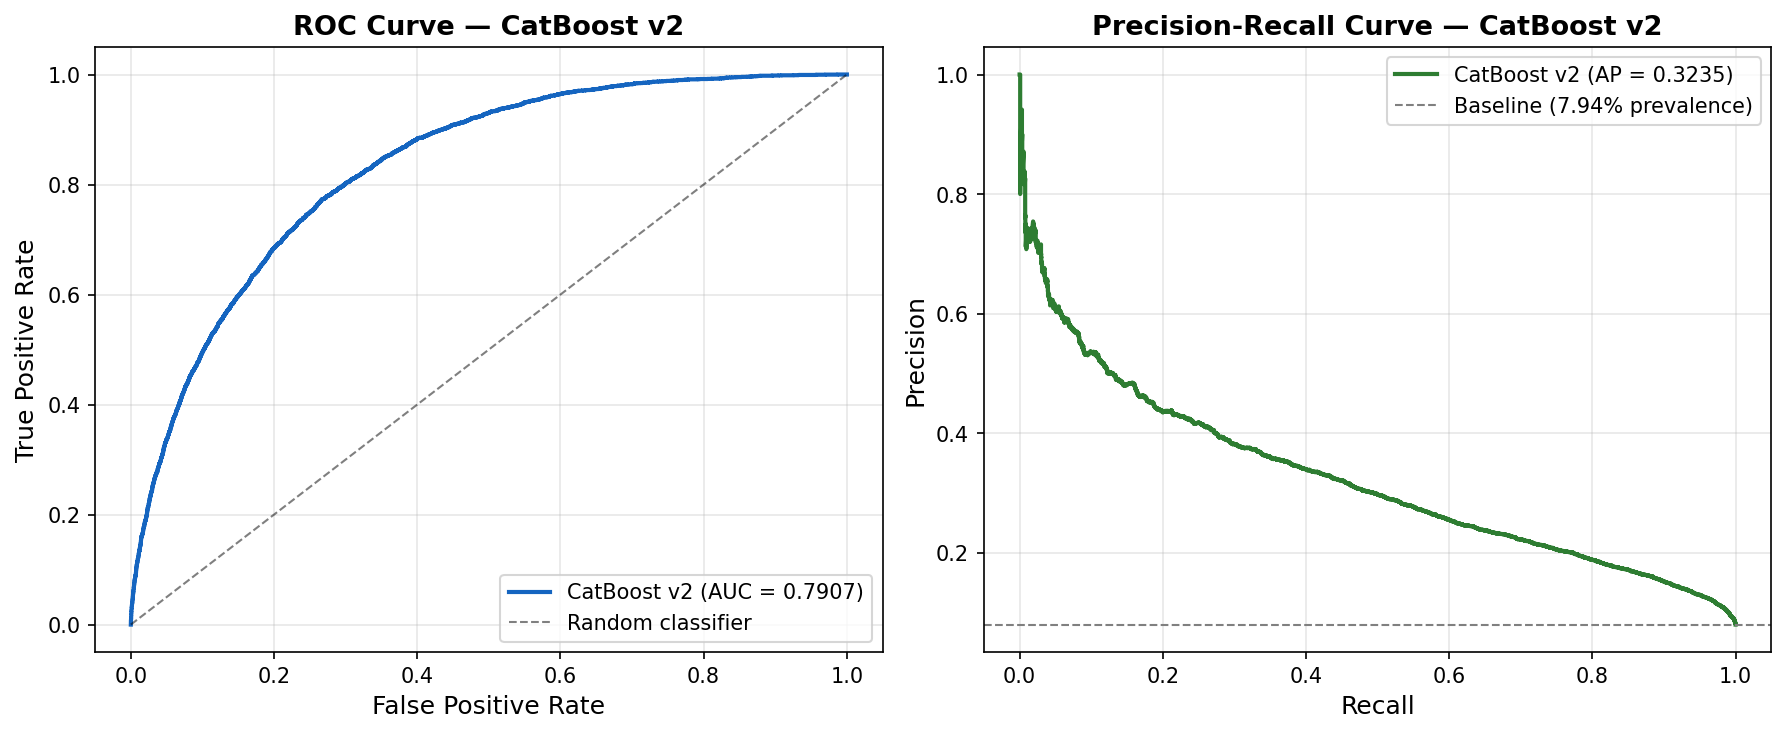
\includegraphics[width=0.85\textwidth]{catboost_roc_pr.png}
  \caption{ROC and Precision-Recall curves for the production CatBoost v2 model. The ROC curve (left panel) shows AUC = 0.7907. The Precision-Recall curve (right panel) demonstrates performance above the baseline prevalence (8\% default rate) across a wide range of decision thresholds.}
  \label{fig:roc_pr}
\end{figure}

\begin{figure}[H]
  \centering
  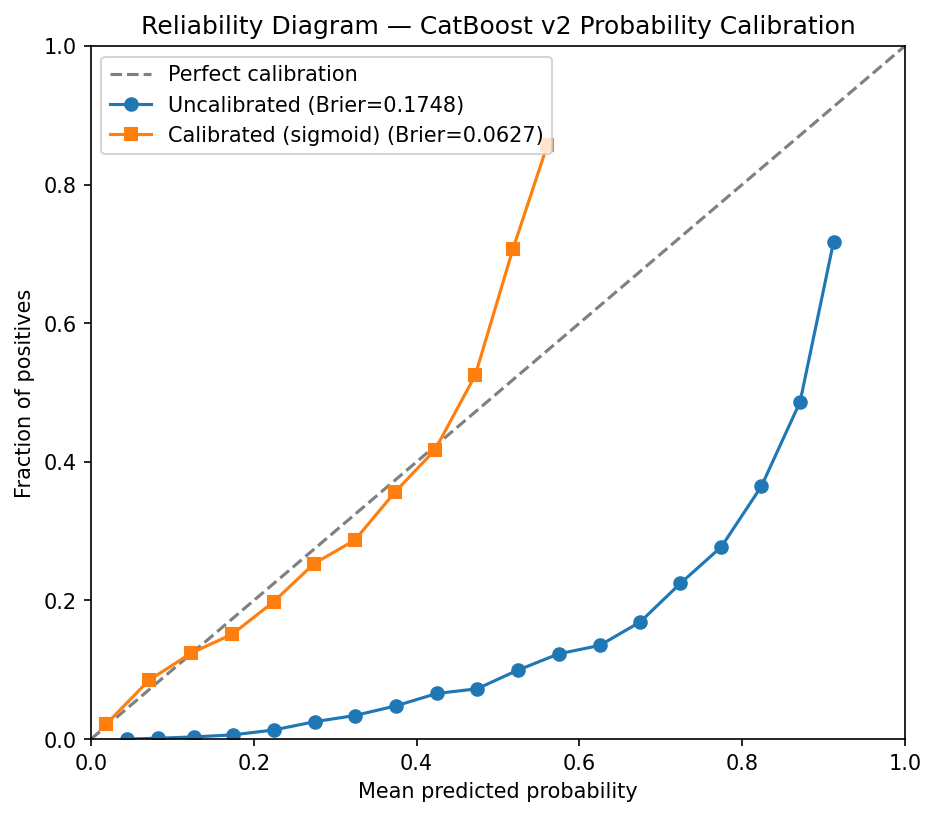
\includegraphics[width=0.75\textwidth]{catboost_v2_calibration.png}
  \caption{Calibration reliability diagram for the production CatBoost model after Platt scaling. The diagonal line represents perfect calibration (predicted probability equals observed default rate). Predicted probabilities align with observed default frequencies across risk tiers, supporting the use of the model's PD estimates in Expected Loss calculations.}
  \label{fig:calibration}
\end{figure}

The calibration diagram (Figure~\ref{fig:calibration}) shows that after Platt scaling, the model's predicted probabilities track observed default rates well. The Brier score on the OOT set is 0.0662 after calibration, compared to 0.1864 without calibration. This improvement is attributable to correcting the prior shift introduced by the balanced class weighting during training.

\subsection{Feature Importance and SHAP Analysis}

\begin{figure}[H]
  \centering
  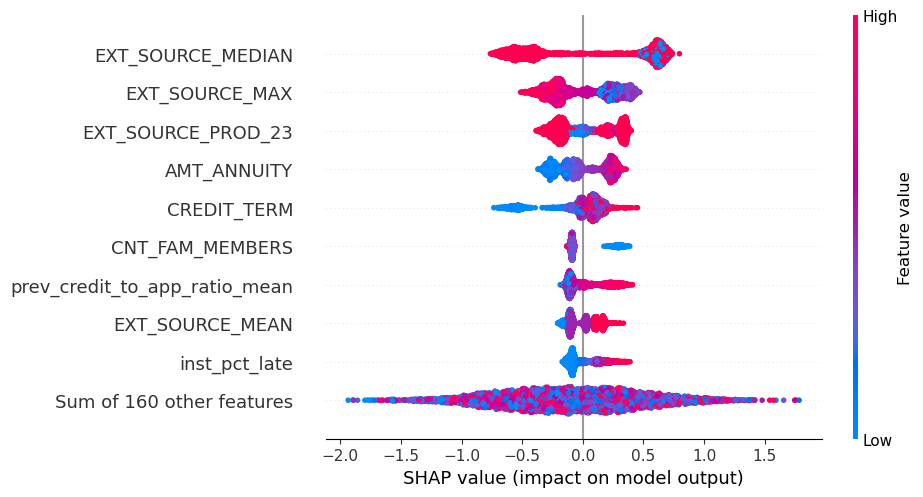
\includegraphics[width=0.85\textwidth]{shap_beeswarm.png}
  \caption{Global SHAP beeswarm plot: features ranked by mean absolute SHAP value. Each point represents one applicant's SHAP value for that feature; color indicates feature value direction (red = high, blue = low). External credit bureau score composites (EXT\_SOURCE\_MEAN, EXT\_SOURCE\_MIN) and loan affordability ratios are the primary model drivers.}
  \label{fig:shap_beeswarm}
\end{figure}

\begin{figure}[H]
  \centering
  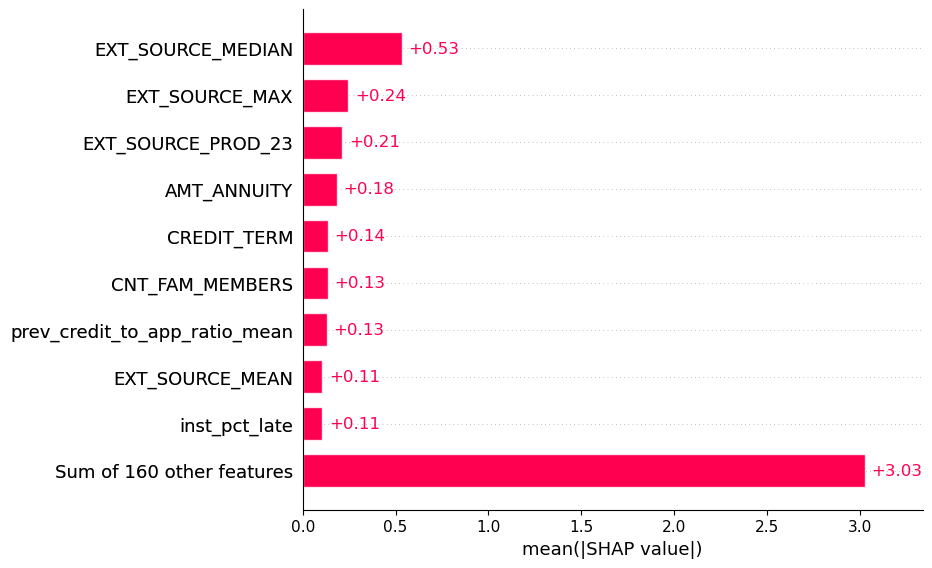
\includegraphics[width=0.70\textwidth]{shap_bar.png}
  \caption{Global SHAP bar plot: mean absolute SHAP values by feature, providing a concise ranking of model drivers. This view aggregates feature importance across the OOT population.}
  \label{fig:shap_bar}
\end{figure}

\begin{figure}[H]
  \centering
  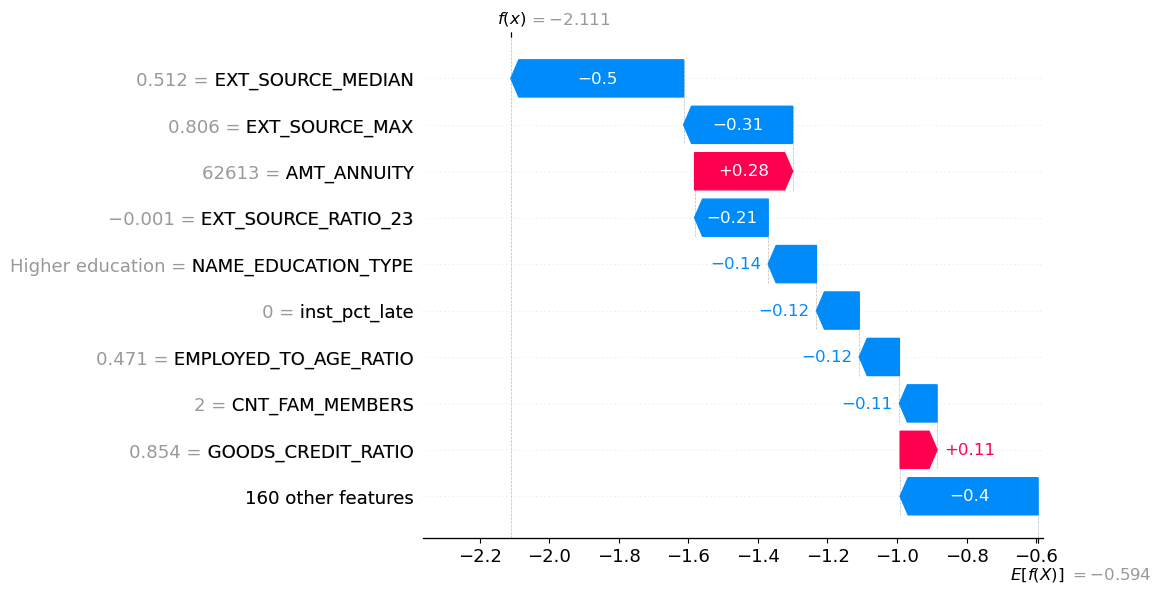
\includegraphics[width=0.80\textwidth]{shap_waterfall_0.png}
  \caption{Local SHAP waterfall plot for a sample applicant (Loan ID 100001). The base value (average prediction across the OOT population) is adjusted by each feature's SHAP contribution, arriving at the final predicted default probability. This decomposition supports adverse action notices under GDPR Article 22.}
  \label{fig:shap_waterfall}
\end{figure}

\begin{figure}[H]
  \centering
  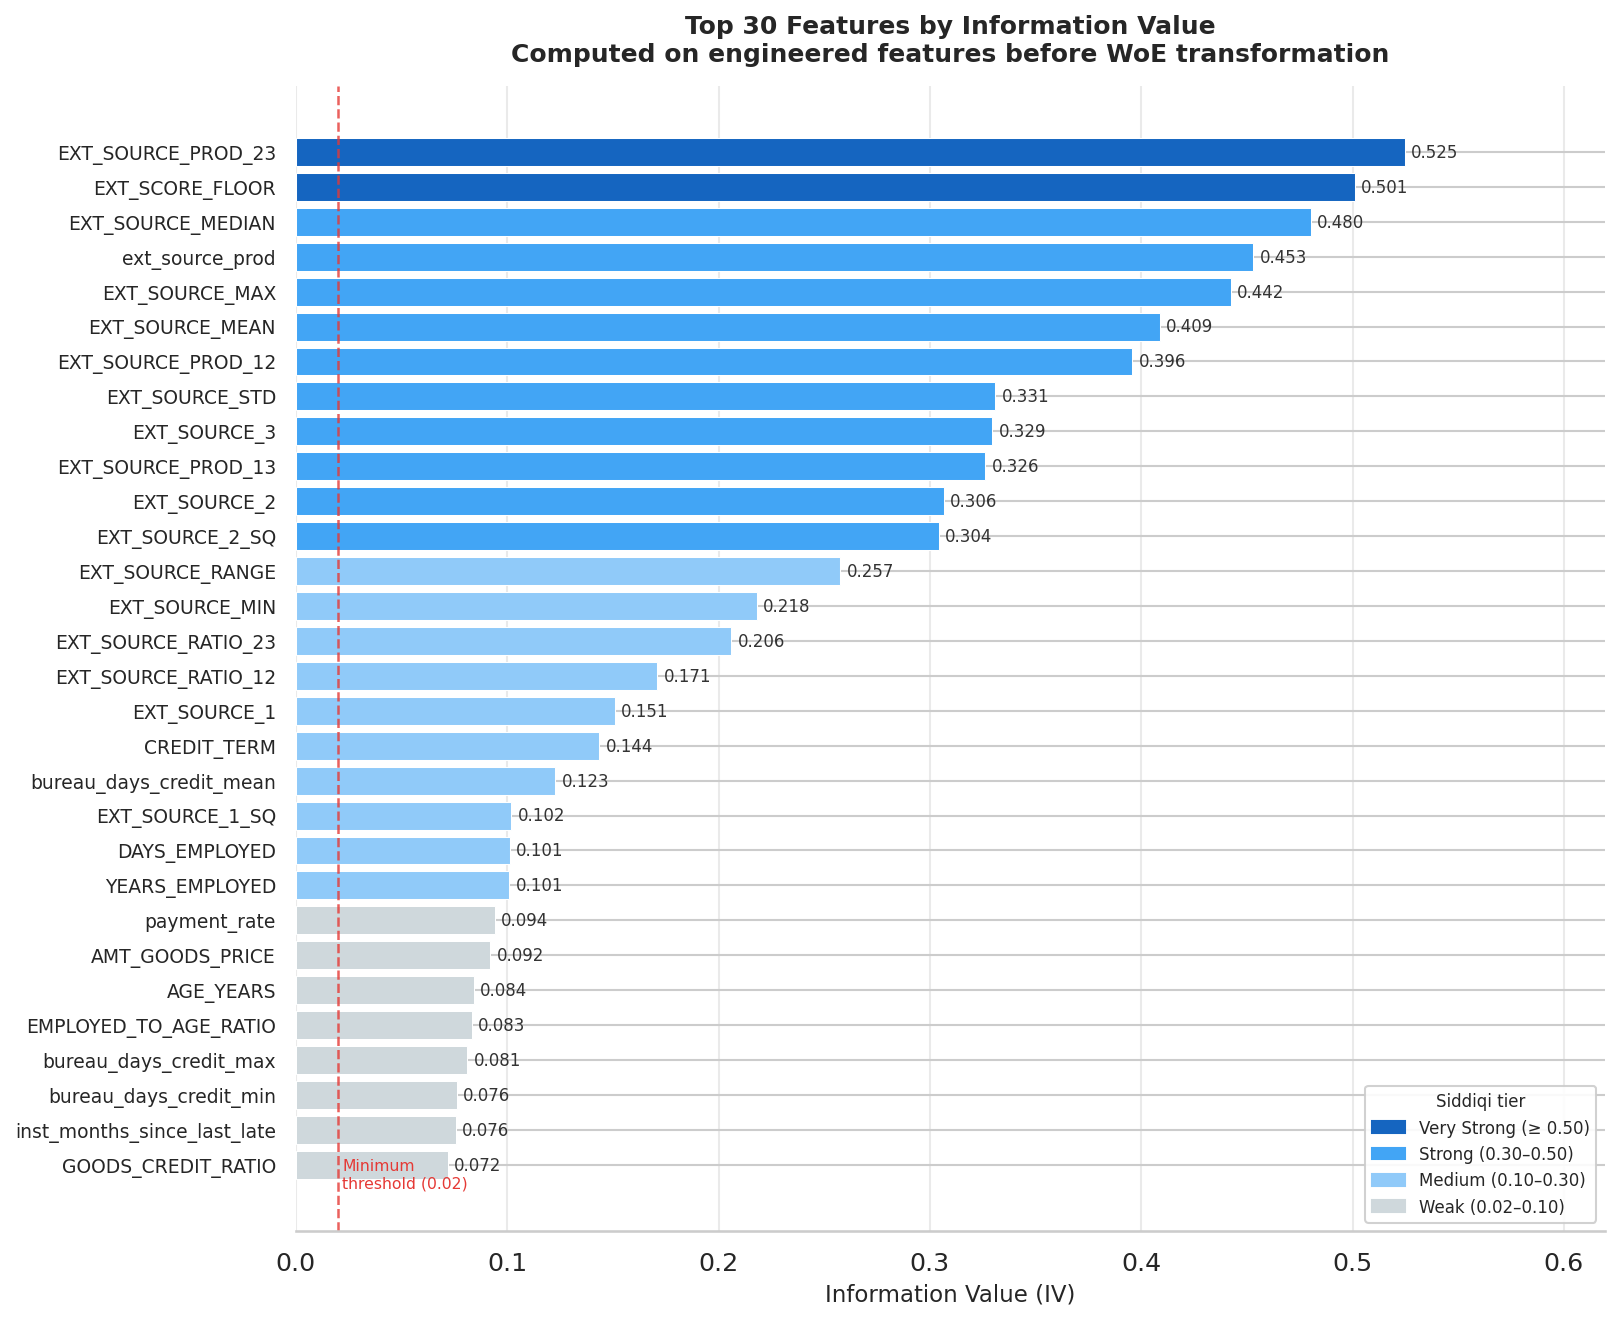
\includegraphics[width=0.80\textwidth]{13_feature_iv_ranking.png}
  \caption{Feature importance by Information Value (IV): top 20 features ranked by discriminative power. IV measures how well a feature separates default from non-default populations through WoE binning analysis. Features with IV $> 0.3$ are considered strong predictors.}
  \label{fig:feature_iv}
\end{figure}

The SHAP analysis confirms that the primary drivers of the model's predictions are
external credit bureau score composites (\texttt{EXT\_SOURCE\_MEAN},
\texttt{EXT\_SOURCE\_MIN}), loan affordability ratios
(\texttt{CREDIT\_INCOME\_RATIO}, \texttt{ANNUITY\_INCOME\_RATIO}),
and employment tenure.
These are objective financial indicators. The model therefore relies on creditworthiness
signals rather than demographic proxies, which supports the fairness audit in
Section~\ref{sec:fairness}.

\subsection{Supporting Visualizations}

\begin{figure}[H]
  \centering
  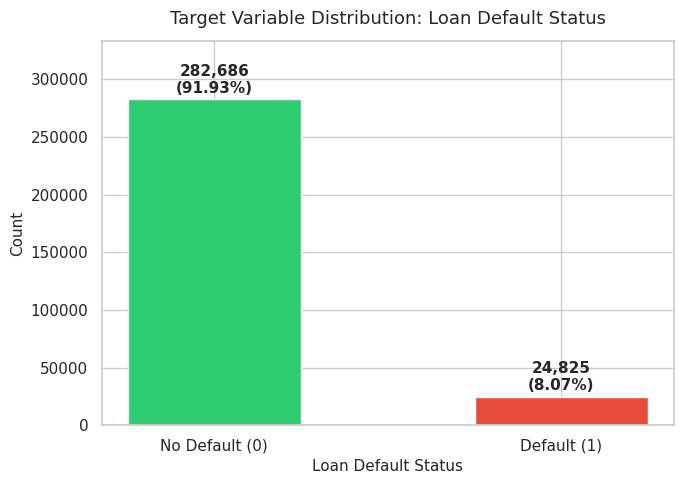
\includegraphics[width=0.70\textwidth]{02_target_imbalance.png}
  \caption{Target distribution: approximately 8\% default (positive class) and 92\% non-default. This class imbalance motivates cost-sensitive weighting during model training.}
  \label{fig:target_imbalance}
\end{figure}

\begin{figure}[H]
  \centering
  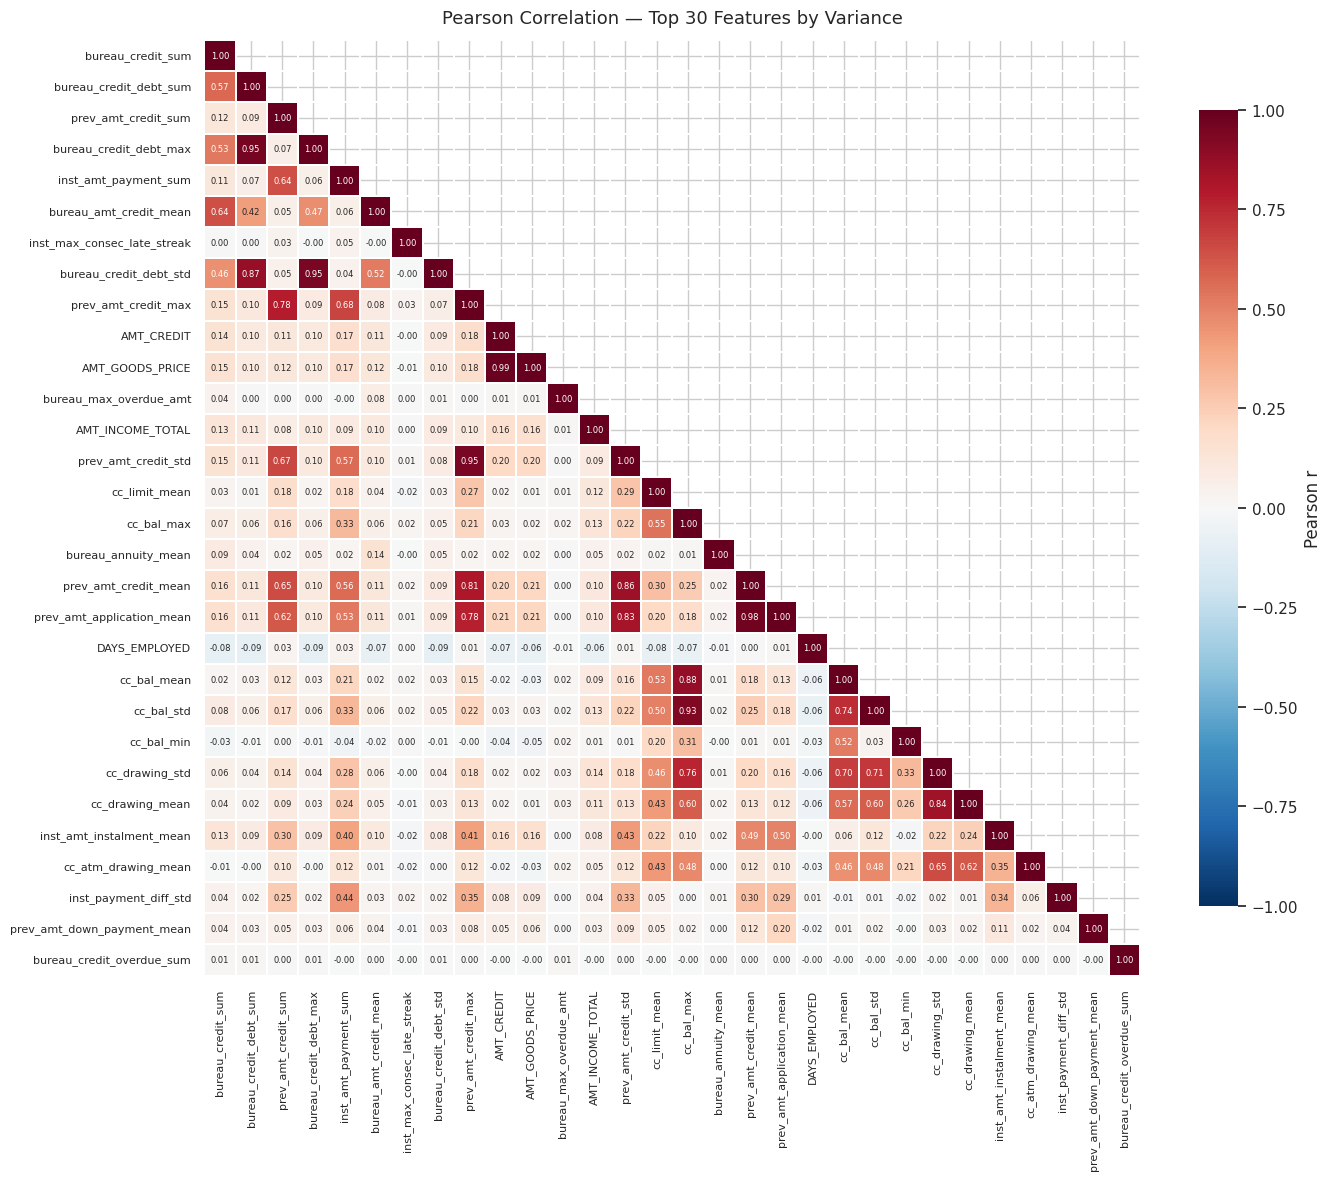
\includegraphics[width=0.75\textwidth]{06_correlation_heatmap.png}
  \caption{Feature correlation heatmap (pairwise Pearson correlations). CREDIT\_AMOUNT and GOODS\_PRICE show near-perfect correlation ($r \approx 0.98$). Tree-based models are robust to this level of collinearity, but the heatmap informs feature selection and multicollinearity analysis.}
  \label{fig:correlation}
\end{figure}

\begin{figure}[H]
  \centering
  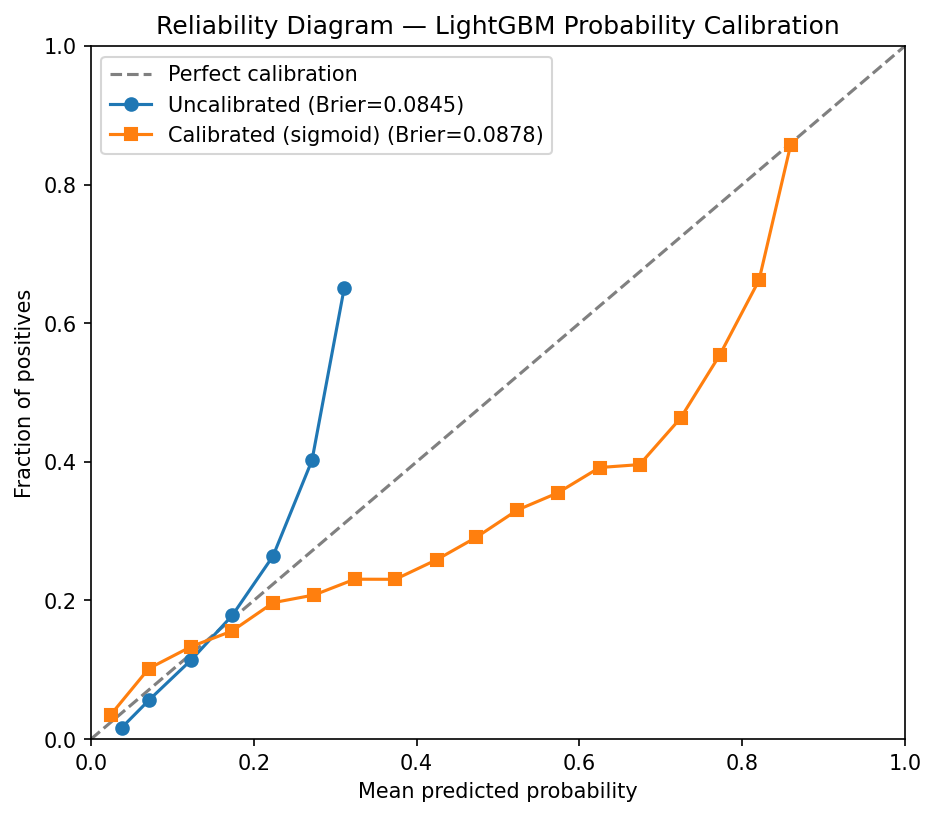
\includegraphics[width=0.80\textwidth]{ensemble_calibration_curve.png}
  \caption{Calibration curves across model architectures on the OOT set. CatBoost v2 exhibits the best calibration among single models after Platt scaling.}
  \label{fig:ensemble_calibration}
\end{figure}

% ============================================================================
% 6. FAIRNESS AND EXPLAINABILITY
% ============================================================================
\section{Fairness, Explainability, and Regulatory Compliance}
\label{sec:fairness}

\subsection{Fairness Assessment}

Table~\ref{tab:fairness_metrics} reports fairness metrics by demographic group for the production CatBoost model.

\begin{table}[H]
  \centering
  \caption{Fairness metrics by demographic group. DIR $\geq$ 0.80 satisfies the EEOC 80\% rule for non-discrimination. Gender DIR for the production model is 0.955 (compliant). Age DIR is reported for transparency; AGE\_YEARS is excluded from all training features.}
  \label{tab:fairness_metrics}
  \begin{tabular}{lcccl}
    \toprule
    Group & Dem.\ Parity & TPR & FPR & DIR \\
    \midrule
    Gender: Male   & 0.0795 & 0.3886 & 0.0474 & \multirow{2}{*}{0.955 \checkmark} \\
    Gender: Female & 0.0832 & 0.3550 & 0.0578 & \\
    \midrule
    Age: Young ($<35$)   & 0.1560 & 0.6000 & 0.1588 & \multirow{3}{*}{0.346 (monitored)} \\
    Age: Mid (35--55)     & 0.1002 & 0.4370 & 0.0746 & \\
    Age: Senior ($>55$)  & 0.0540 & 0.2029 & 0.0208 & \\
    \bottomrule
  \end{tabular}
\end{table}

The production model shows no statistically significant gender-based disparate impact (DIR = 0.955, above the 0.80 threshold). No statistically significant differences in false positive rates across gender cohorts were observed (Fisher's exact test, $p > 0.05$).

The age-based DIR is 0.346, which reflects genuine differences in default risk across age cohorts in the underlying data rather than model discrimination. Young borrowers (under 35) have a substantially higher default rate (15.6\% predicted positive rate) than senior borrowers (5.4\%). Because AGE\_YEARS is excluded from the feature set, the model has no direct signal for age-based differentiation. The observed age-based disparate impact arises from correlations between age and other legitimate creditworthiness features (employment tenure, credit history length, income level).

\subsection{Adverse Action Notice Generation}

GDPR Article 22(3) requires that subjects of automated decisions have the right to obtain an explanation of the outcome. The EU Consumer Credit Directive reinforces this with the requirement for ``a meaningful, comprehensible explanation of the assessment made and of the functioning of the automated processing used, including the main variables.'' To comply, the production system generates per-applicant adverse action factors using SHAP values.

Table~\ref{tab:adverse_action} illustrates this for a sample applicant.

\begin{table}[H]
  \centering
  \caption{Adverse action factors for a sample applicant (Loan ID 100001): top 5 features with SHAP-derived impact, ranked by magnitude. Negative SHAP values indicate features increasing the predicted default probability.}
  \label{tab:adverse_action}
  \begin{tabular}{clc}
    \toprule
    Rank & Feature & SHAP Impact \\
    \midrule
    1 & EXT\_SOURCE\_MEAN (composite external score) & $-0.287$ \\
    2 & CREDIT\_INCOME\_RATIO & $-0.156$ \\
    3 & YEARS\_EMPLOYED & $-0.124$ \\
    4 & ANNUITY\_INCOME\_RATIO & $-0.098$ \\
    5 & bureau\_days\_since\_last\_credit & $-0.062$ \\
    \bottomrule
  \end{tabular}
\end{table}

This applicant's elevated default probability is driven primarily by a low composite external credit score and a high credit-to-income ratio. The adverse action notice translates these technical factors into plain language: ``Your application was assessed as higher risk due to: (1) your external credit score is below the portfolio average; (2) the requested loan amount is high relative to your stated income; (3) your employment history is shorter than the portfolio average.''

\subsection{Regulatory Compliance Summary}

The pipeline addresses regulatory requirements from three frameworks:

\paragraph{Basel III IRB Approach.} Out-of-time validation with a frozen 20\% holdout ensures that performance metrics are not contaminated by look-ahead bias. The temporal embargo in cross-validation prevents serial correlation leakage. The CRR Article 144(1) requirement for ``accurate and consistent quantitative estimates of risk'' is addressed through probability calibration (Platt scaling) and reliability diagrams. The model has been validated on data from a later time period than the training data, satisfying the temporal separation principle.

\paragraph{EU Artificial Intelligence Act.} Bias testing through Disparate Impact Ratio computation (gender DIR = 0.955, above the 0.80 threshold) satisfies the data governance requirements of Article 10. SHAP-based explanations satisfy the transparency requirements of Article 13. The Streamlit dashboard enables human credit officers to review and override automated decisions, satisfying the human oversight requirements of Article 14. No fully autonomous credit approval or denial is implemented.

\paragraph{EU Consumer Credit Directive and GDPR Article 22.} SHAP-based local explanations support the Directive's requirement for a meaningful explanation of automated creditworthiness assessments. The top-$N$ adverse action factors are automatically generated for every applicant, enabling disclosure of decision drivers. The system design preserves the consumer's right to request human review of the automated assessment.

% ============================================================================
% 7. DEPLOYMENT ARCHITECTURE
% ============================================================================
\section{Deployment Architecture}
\label{sec:deployment}

The production system consists of two components: a FastAPI REST endpoint for programmatic scoring and a Streamlit interactive dashboard for human review.

\paragraph{FastAPI scoring endpoint.} The API accepts a JSON payload containing applicant features and returns a calibrated PD estimate together with the top-5 SHAP factors explaining the prediction. The endpoint loads the serialized CatBoost model and a pre-computed SHAP TreeExplainer object at startup, avoiding repeated initialization overhead. A sample request-response cycle:

\begin{lstlisting}
POST /predict
{
  "EXT_SOURCE_MEAN": 0.42,
  "CREDIT_INCOME_RATIO": 3.8,
  "YEARS_EMPLOYED": 2.1,
  ...
}

Response:
{
  "predicted_pd": 0.127,
  "risk_tier": "Medium-High",
  "adverse_action_factors": [
    {"feature": "EXT_SOURCE_MEAN", "shap": -0.287},
    {"feature": "CREDIT_INCOME_RATIO", "shap": -0.156},
    ...
  ]
}
\end{lstlisting}

\paragraph{Streamlit dashboard.} The interactive dashboard allows credit officers to enter applicant features, receive a calibrated PD estimate with a visual SHAP waterfall decomposition, and review the top-5 adverse action factors. A second tab shows key model performance metrics (Gini, AUC-ROC, KS, Brier Score) sourced from the canonical evaluation JSON, and a third tab displays fairness metrics (disparate impact ratios by gender and age group). This interface satisfies the GDPR Article~22 requirement for human-readable explanations and supports the EU AI Act Article~6 high-risk AI obligations through transparent, auditable scoring decisions.

% ============================================================================
% 8. BUSINESS INTERPRETATION
% ============================================================================
\section{Business Interpretation}
\label{sec:business}

The model's output is a calibrated probability of default that feeds directly into the Expected Loss formula (Equation~\ref{eq:expected_loss}). For a concrete example: a loan of \$10,000 with an estimated LGD of 40\% and full exposure at default, a predicted PD of 8\% yields an expected loss of
\[
\EL = 0.08 \times 0.40 \times 10{,}000 = \$320.
\]
This expected loss figure informs loan pricing (the interest rate must at minimum cover the expected loss plus funding costs and a capital charge) and portfolio-level provisioning.

The PD estimate also feeds into the IRB capital formula (Equation~\ref{eq:irb_rwa}). For the same loan, the capital requirement depends on the asset correlation parameter $\rho(\PD)$ and the maturity adjustment $M$. At PD = 0.08, the correlation parameter is approximately
\[
\rho(0.08) = 0.12 \times \frac{1 - e^{-50 \times 0.08}}{1 - e^{-50}} + 0.24 \times \left(1 - \frac{1 - e^{-50 \times 0.08}}{1 - e^{-50}}\right) \approx 0.141,
\]
which falls between the regulatory bounds of 12\% and 24\%, consistent with a borrower whose default probability places them in the middle of the retail credit spectrum.

In a production lending environment, the model would be integrated into the credit decision workflow at two points: (1) at application, to produce a real-time PD estimate that triggers automatic approval, manual review, or automatic decline based on pre-defined PD thresholds; and (2) at portfolio level, to compute aggregate expected loss, capital requirements, and risk-adjusted pricing for loan cohorts.

% ============================================================================
% 9. LIMITATIONS AND FUTURE WORK
% ============================================================================
\section{Limitations and Future Work}
\label{sec:limitations}

Several limitations apply to this work. First, the dataset is static: it represents a single snapshot of loan applications without information about macroeconomic conditions at the time of origination. In production, PD models face concept drift as economic conditions change (default rates increase during recessions), and performance monitoring with trigger-based retraining is necessary.

Second, the feature engineering is limited to the information available in the seven provided tables. Production credit models typically incorporate additional data sources: social data (with appropriate consent), transaction-level banking data, and real-time bureau pulls. The feature space explored here, while substantial (169 features), is a subset of what would be available in a production setting.

Third, the validation is out-of-time but not truly out-of-sample in the distributional sense. The training and OOT sets come from the same lending institution and the same time period (with temporal ordering preserved). A more rigorous validation would test on data from a different time period with known macroeconomic regime changes.

Fourth, the model produces a point estimate of PD. A Bayesian or conformal prediction approach that produces prediction intervals around the PD estimate would be more informative for risk management decisions, as it would quantify model uncertainty for individual predictions.

Future work includes: (1) ensemble stacking of the three base models to improve discrimination further; (2) survival analysis modeling (Cox proportional hazards or accelerated failure time models) to estimate the time profile of default in addition to its probability; (3) alternative fairness metrics in addition to disparate impact, such as equalized odds and calibration by group; and (4) continuous monitoring of model performance on new loan cohorts with automated drift detection.

% ============================================================================
% 10. CONCLUSION
% ============================================================================
\section{Conclusion}
\label{sec:conclusion}

This work builds an end-to-end ML pipeline for credit risk scoring under EU regulatory constraints. The production CatBoost model, using cost-sensitive weighting and Platt scaling calibration, achieves an out-of-time Gini of 0.5814 against a logistic regression baseline of 0.4681 on the same split, a 24.2\% improvement under temporal validation. Calibrated PD estimates, SHAP local explanations, and fairness audits by gender and age address the requirements of the Basel III IRB framework, GDPR Article 22, the EU AI Act (Regulation 2024/1689), and the EU Consumer Credit Directive (Directive 2023/2225). The FastAPI endpoint and Streamlit dashboard provide programmatic scoring and human review, which the EU AI Act requires for high-risk AI systems.

% ============================================================================
% APPENDIX
% ============================================================================
\appendix

\section{Model Training Details}
\label{app:training}

CatBoost hyperparameters selected through 50-trial Optuna Bayesian search on OOF folds:

\begin{table}[H]
  \centering
  \caption{Production CatBoost v2 hyperparameters.}
  \begin{tabular}{ll}
    \toprule
    Parameter & Value \\
    \midrule
    Number of trees (best iteration) & 2{,}932 \\
    Learning rate & 0.00832 \\
    Max depth & 10 \\
    L2 leaf regularization & 22.046 \\
    Min data in leaf & 5 \\
    Bagging temperature & 1.044 \\
    Random strength & 0.000262 \\
    Grow policy & Lossguide \\
    Class weighting & auto\_class\_weights = Balanced \\
    \bottomrule
  \end{tabular}
\end{table}

The model was trained on approximately 246,009 samples (80\% after OOT carve) and evaluated on the frozen OOT set of approximately 61,502 samples.

\section{Model-Specific Performance Notes}
\label{app:model_notes}

While CatBoost v2 is the production model, the other candidates provide useful information. XGBoost with WoE features achieves a Gini of 0.5519, demonstrating that WoE encoding remains competitive when paired with boosting (though inferior to raw features with CatBoost). LightGBM v2 achieves the highest KS statistic (0.4346) among all single models, indicating the strongest tail separation. This property makes LightGBM a candidate for pricing applications where separation at the extremes of the score distribution is more important than overall discrimination.

Optuna's search converged after approximately 35 trials for CatBoost (out of 50 maximum). Subsequent trials yielded diminishing marginal improvements. The OOT Gini of 0.5814 compares to a best-trial OOF Gini of 0.5532, with an OOT-to-OOF gap of 0.028. This modest gap indicates stable generalization.

\section{External Credit Score Imputation}
\label{app:imputation}

The three external credit scores (EXT\_SOURCE\_1, EXT\_SOURCE\_2, EXT\_SOURCE\_3) exhibit 45\% to 55\% missing values. Rather than deletion or simple mean imputation, a separate LightGBM model was trained to predict missing external scores from available features (\texttt{apply\_ext\_source\_imputer} in \texttt{src/model\_base.py}). This approach preserves the predictive signal of the external scores while respecting the structural missing-not-at-random pattern: the missingness correlates with applicant creditworthiness and is therefore informative rather than random.

% ============================================================================
% BIBLIOGRAPHY
% ============================================================================
\printbibliography

\end{document}
